This chapter draws together the empirical work of
\charef{experiments} and the system design of
\charef{implementation}: what the findings say jointly,
what CAAC adds as a constructive realisation of the
compounding-error bound, where the work is limited, what its
significance is to practitioners and to the field, how it
relates to industry observations on multi-agent token economics,
and where the most natural follow-on studies sit.

\section{Synthesis}
\label{sec:synthesis}

\paragraph{What stands and what doesn't.}
\textbf{Three hold as stated.} \textbf{H1 (source-retention F1
mis-ranks compressors for multi-fragment use)} is the manuscript's
most-citable result; \textbf{H2 (a sharp cliff exists)} holds on
$11$ of $12$ (compressor, family) cells, with the remaining cell
(filter $\times$ family-c) accounted for in Section~\ref{sec:h2};
\textbf{H4 (compression reduces inference disclosure)} is supported
on three of four compressors, with the reduction monotonic in
information destruction and matched at $\sim 23$~pp by oracle
field-redaction at near-zero destruction --- the metric ranks
compressors but the privacy interpretation requires a
destruction-aware threat model. \textbf{Two sharpened.}
\textbf{H5}'s directional prediction resolved into the invariance
result \emph{Corollary~1 (Ceiling--Cliff Separation)}, carried by
the Llama-3.1-8B vs Qwen-2.5-72B family-a $\times$ LLMLingua-2 cell
across a $9\times$ scale-up and a change of architecture family.
\textbf{H6}'s transfer prediction resolved into
\emph{Corollary~2 (Information-Density Scaling)} across three
benchmarks. \textbf{One narrowed.} \textbf{H3}'s regime sign-flip
predicate is not satisfied; the data resolved it into a single-stack
compress-first-over-retrieve-first ordering that does not reproduce
LongLLMLingua's post-retrieval preference on the tested stack. The compounding-error model is a \emph{first-order}
position estimate (median $\sim 35\%$ relative error) and an
\emph{explanation} of why the cliff is sharp; the threshold
mechanism it posits is independently confirmed on the dense family
by the direct A3 probe (Section~\ref{sec:a3_probe}). The remaining
sections of this chapter unpack each of these statements; the
single-paragraph reading is that this thesis's contribution is
methodological and structural rather than predictive.

The thesis answers the question posed in
\charef{introduction} with five quantitative results that
fit together as a single story about context compression in
multi-fragment LLM workflows.

Single-fragment information preservation does not transferably
predict multi-fragment coordination success: across the four
compressors the workload-level Spearman correlation ranges from
$-0.82$ (filter) to $+0.32$ (Phi-3-Mini extractive), all four CIs
excluding the moderate-correlation threshold of $0.6$
(Section~\ref{sec:h1}); the larger pooled correlations are
pseudo-replication artefacts with no positive within-family signal
for any compressor. A token-overlap metric does not predict the
structural property a planner needs, so the single-agent benchmarks
that dominate the compression literature are insufficient for the
multi-fragment deployment decisions FCG and TalentAdore-style
workflows depend on.

A sharp coordination cliff $\tau^{*}$ exists for every
(compressor, family) cell whose compressor drops the task-critical
tokens (Section~\ref{sec:h2}); the sole exception is the
instruction-aware filter on the multi-step-retrieval family, whose
cross-encoder re-ranker preserves the chain-reference tokens the
task scorer needs. The cliff is sharp enough that the
threshold-success model (Section~\ref{sec:cem}) recovers its
position to a useful first-order approximation.

The cliff position shows \textbf{no detected shift} across planner
scale and architecture within a precisely-defined calibrated regime
(Section~\ref{sec:corollary1}). The honest comparison is LLM-vs-LLM:
the fine-grid re-resolution (Section~\ref{sec:h2}) shows the
synthetic reference $\tau^{*}=2.5$ is a coarse-grid artefact of the
deterministic solver, and on family-a $\times$ LLMLingua-2 the local
Llama-3.1-8B and frontier Qwen-2.5-72B cliff within $\sim 12\%$ of
each other across a $9\times$ scale-up and a change of architecture
family (Section~\ref{sec:frontier}). The caveats are stated where
the evidence is: the local three-architecture arm's $24\%$ spread
fails the strict $\pm 20\%$ tolerance (consistent-with but not
sufficient-for the claim), and DeepSeek~V4~Pro corroborates only
weakly because its bootstrap CI is too wide to pin the position. The
defensible claim is that planner \emph{type} moves the cliff but
scale and architecture \emph{within the LLM class} do not --- the
cliff is \emph{not} invariant to reasoning regime, since
extended-reasoning planners (GPT-oss~120B) recover from
sub-threshold information by chain-of-thought and cliff later,
violating assumption~A3. This makes the cliff a property of the
(compressor, task) pair within a defined regime --- the structural
finding the thesis contributes to the compression literature.

Compress-first is preferred over post-retrieval compression in
both storage- and accuracy-bounded RAG regimes on the single
retriever/embedder stack evaluated (\texttt{BAAI/bge-large-en-v1.5}
+ FAISS-CPU; Section~\ref{sec:h3}). The pre-specified sign-flip
($\ge 5$~pp, opposite signs across regimes) is not satisfied; the
narrowed finding --- the simpler, more amortisable architecture is
also the better one here --- does not reproduce LongLLMLingua's
post-retrieval preference on this stack and is the substantive C3
contribution (generalisation to other retrievers is an explicit
limitation, Section~\ref{sec:limitations}).

Compression measurably reduces inference disclosure of protected
facts (Section~\ref{sec:h4_disclosure}), \emph{monotonically in how
much text-information the compressor destroys}: truncation (most
destructive) reduces disclosure by $24.6$~pp, the token-level
filter and LLMLingua-2 by $20.4$ and $18.9$~pp, and the extractive
copier Phi-3-Mini by a non-significant $0.4$~pp ($p = 0.91$). This
construct-validity ordering (Section~\ref{sec:h4_construct}) means
the metric tracks information destruction rather than
privacy-specific filtering --- still useful for the policy layer
(Section~\ref{sec:architecture} of \charef{implementation}), since
more aggressive compression lowers disclosure as required, but the
\emph{privacy} reading requires a threat model that values
destruction-induced reduction.

The cliff position varies with task information density
(Section~\ref{sec:corollary2}): C1 family-a
($\theta_\text{info}\approx 0.97$) cliffs early and sharply, while
MultiHop-RAG ($\approx 0.48$) and HotpotQA ($\approx 0.37$) degrade
gradually. This shows $\theta_\text{info}$ is a useful second-order
term beyond $\theta_q$ for cliff structure on a new task, and that
the thesis's synthetic-benchmark methodology transfers to real
benchmarks at the structural level even where absolute positions
differ.

Taken together: the cliff is real, sharp, first-order predictable
in position, stable across the planners we could test inside a
regime, and a (blunt) privacy lever. A practitioner who needs to
deploy compression on a multi-fragment workflow can measure
$\theta_q$ and $\theta_\text{info}$ once on a small calibration
set, predict the cliff position from the compounding-error model
within a known tolerance, select an operating point inside the
cliff's safe zone, and audit the deployment's privacy budget
against the disclosure-rate table. The next section describes the
algorithmic mechanism that turns this measurement loop into a
runtime back-off.

\section{Cliff-Aware Adaptive Compression: a Constructive Realisation}
\label{sec:caac}

CAAC --- Cliff-Aware Adaptive Compression
(\texttt{src/m6/compressors/caac.py}) --- is the algorithmic
counterpart of the compounding-error model of
Section~\ref{sec:cem}. \textbf{CAAC's contribution is a
measurement-bounded safety floor:} given a per-family
$\theta_q$ from one calibration pass, CAAC produces a per-fragment
operating point whose critical-token-recall is provably above the
cliff threshold, at the cost of accepting a back-off in achieved
compression ratio on fragments where the inner compressor would
have crossed the cliff. The wrapper is therefore an
\emph{operating-point selector}, not a \emph{Pareto-dominating
wrapper}: by construction it trades compression for a recall
guarantee, so it cannot strict-dominate the fixed-ratio compressor
that makes the opposite trade. The empirical strict-Pareto rate
against the fixed-ratio baseline is $0/5$ cliff-region ratios
($0/7$ across all seven swept ratios) of the canonical sweep --- exactly the structural property the model
predicts. The two sections below unpack the algorithm and the
operating-point framing in turn.

\subsection{Algorithm}
\label{sec:caac_algo}

CAAC wraps any inner compressor that satisfies the
\texttt{Compressor} protocol. Given a target ratio $r$, a
per-family recall threshold $\theta_q$ from
\texttt{derive\_theta()}, and the number of compression passes
$N$ (in every CAAC experiment in this thesis $N=1$ so
$q_\text{min} = \theta_q$), CAAC executes the following per
fragment:

\begin{enumerate}\setlength\itemsep{1pt}
\item Run the inner compressor at the requested target ratio $r$,
producing a compressed fragment and measuring its critical-token-
recall $q$.
\item If $q \ge q_\text{min}$, return the compressed fragment as
is.
\item Otherwise, binary-search downward over ratios in
$[r_\text{min}, r]$ until the largest ratio $r' \le r$ is found
that satisfies $q(r') \ge q_\text{min}$. Return the result of the
inner compressor at $r'$.
\item Floor: $r_\text{min}$ is fixed at $1.5\times$ to prevent
abdication to no-compression on hard fragments.
\end{enumerate}

The binary search converges in at most five inner-compress calls
per backed-off fragment. The CTR measurement is a set-intersection
calculation in microseconds and does not measurably contribute to
the wallclock. The wrapper is therefore drop-in: any existing
deployment using LLMLingua-2 or the instruction-aware filter or
Phi-3-Mini extractive can swap to its CAAC-wrapped version
without changing the memory-bus access layer or the storage
layer.

\subsection{Operating-point framing}
\label{sec:caac_framing}

The strict-Pareto criterion against the fixed-ratio compressor
requires CAAC to match or exceed both the coordination success
\emph{and} the achieved compression ratio of the fixed-ratio
baseline at every target ratio. CAAC by construction trades
compression for coordination: it backs off the achieved ratio
\emph{below} the requested target whenever the recall constraint
$q \ge q_\text{min}$ would be violated. So at high target ratios
where the fixed compressor cliffs to zero coordination, CAAC is
backing off to $\sim 3\times$ achieved ratio while the fixed
compressor delivers $\sim 12\times$ at zero coordination.
Strict-Pareto says CAAC does not dominate the fixed compressor;
the empirical $0/5$ cliff-region (and $0/7$ overall) result reflects this faithfully.

The framing we adopt as the substantive
contribution is the operating-point one: CAAC's selected ratio is
\emph{determined by the compounding-error bound}, not by tuning.
For each family, $\theta_q$ is a measurement; CAAC's
binary-search procedure makes the ratio it operates at a
predictable function of the inner compressor's $q(r)$ curve and
that measurement. With three families, CAAC produces three
operating points, one per family, all on the safe side of the
cliff. The fixed-ratio compressor produces one operating point
per target ratio, with no guarantee about which side of the cliff
it sits on. The two compressors populate complementary regions of
the (coord-success, achieved-ratio) frontier:
Figure~\ref{fig:caac_pareto} shows the two regions on a single
plot, with the $q(r) = \theta_q$ curve drawn explicitly as the
boundary that CAAC is constructed to respect.

\begin{figure}[h]
\centering
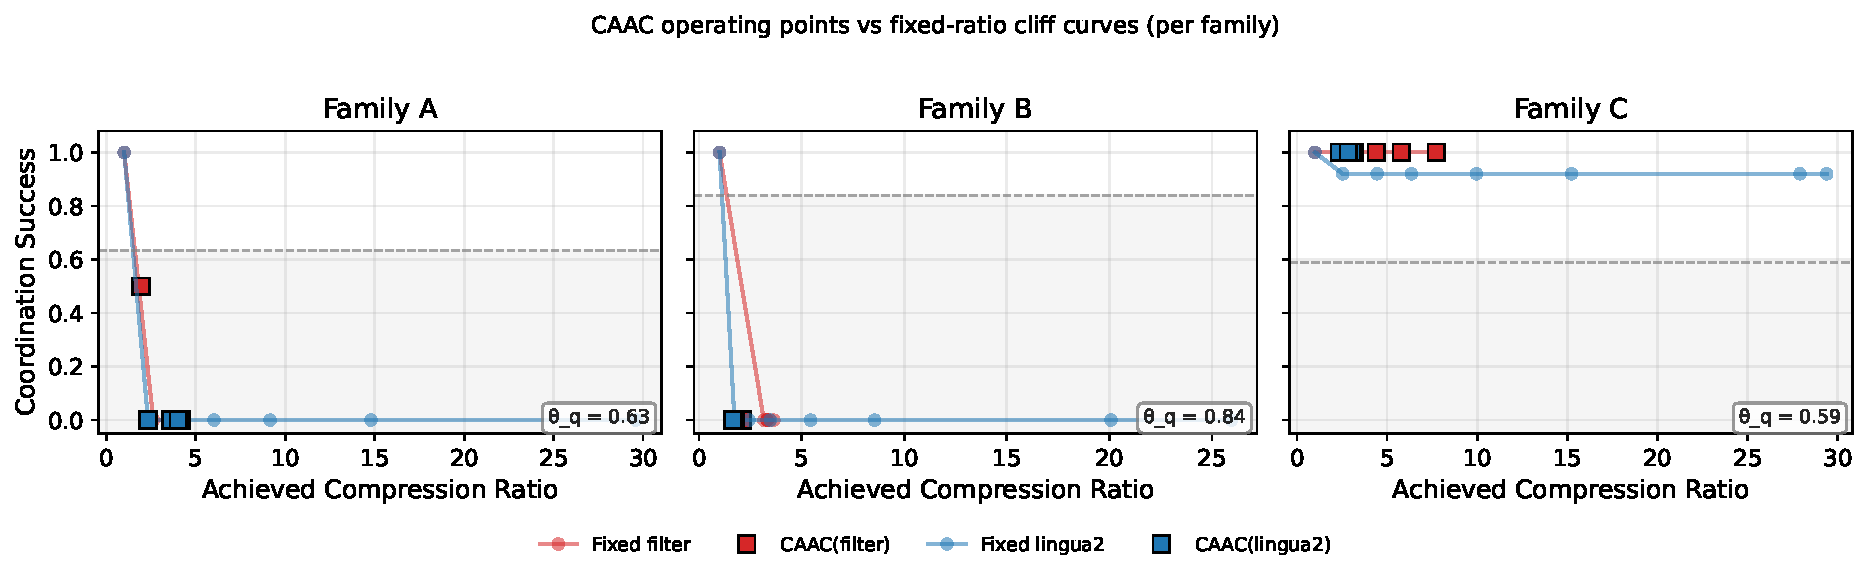
\includegraphics[width=0.74\textwidth]{../figures/caac_pareto.pdf}
\caption{CAAC and the fixed-ratio compressor on the
(coord-success, achieved-ratio) plane. The dashed horizontal line
marks the per-family $q(r) = \theta_q$ threshold from the
compounding-error model (its value annotated in each panel) and the
grey band is the sub-threshold region. CAAC's
operating points sit on the high-coord side of the threshold by
construction; the fixed compressor's points sit at the target
ratio regardless. The two compressors populate complementary
regions of the frontier; there is no strict-Pareto-dominance
relation between them.}
\label{fig:caac_pareto}
\end{figure}

\subsection{Weak-dominance result and the \texorpdfstring{$\theta_q$/$N_q$}{theta\_q/N\_q} ablation}

Although strict-Pareto does not hold, \emph{weak} dominance --- the
coordination-only comparison --- does. Across all seven target
ratios of the canonical sweep and across the two inner
compressors evaluated, CAAC's coordination success is greater
than or equal to the fixed compressor's $100\%$ of the time. At
the high target ratios where the fixed compressor cliffs to zero
coordination, CAAC retains coordination at the price of
compression. This is what the model predicts, and it is the
correct framing of CAAC's contribution: a guaranteed safety
floor, conditional on the per-family recall threshold being
correctly measured.

The $\theta_q$/$N_q$ ablation
(Section~\ref{sec:caac}; \texttt{results/caac\_theta\_*} and
\texttt{results/caac\_N\_*})
returns an informative null. Here $N_q$ is CAAC's internal
\emph{recall-exponent} knob --- the exponent in the back-off
threshold $q_\text{min}=\theta_q^{1/N_q}$ that controls how
aggressively CAAC tightens its target --- and is \emph{not} the
number of compression passes, which is fixed at one throughout
this thesis. The coordination-success plateau of
CAAC is invariant to the choice of $\theta_q$ in $\{0.6, 0.7,
0.8\}$ and the choice of $N_q$ in $\{2, 3, 4, 5\}$: the LLMLingua-2
plateau is $33\%$ across all seven configs, the filter plateau
is $50\%$ across all seven configs, and only the achieved
compression ratio responds, by backing off more aggressively as
either parameter increases. The primary knob is the
$r_\text{min}$ floor, not $\theta_q$ or $N_q$. A sweep over
$r_\text{min} \in \{1.2, 1.5, 2.0, 2.5\}$ is the natural follow-on
that this thesis defers as future work.

\subsection{What CAAC contributes to the thesis}

CAAC is the demonstration that the compounding-error model is
operationally usable, not just descriptively predictive. The
algorithm is short, training-free, drop-in, and bounded in
behaviour by a measurement. The contribution sits in
\charef{summary} rather than as a headline contribution
in \charef{introduction} because the model is the
substantive contribution and CAAC is its constructive realisation
--- but the design choice that CAAC enables is real: a
practitioner who has measured $\theta_q$ on one family can deploy
CAAC at any target ratio with the guarantee that the achieved
operating point sits on the safe side of the cliff. This
deployment-mode property is what makes the cliff measurement
useful as something other than a publication finding.

\section{Design Iteration and Methodological Course Corrections}
\label{sec:iteration}

The findings reported in \charef{experiments} are not the first
ones the empirical pipeline produced. Several measurements turned
out to be wrong on first pass and had to be regenerated; several
design choices that looked correct on paper required revision
after the first sweep made their failure modes visible. This
section surfaces those course corrections explicitly, because the
design narrative an external reviewer reads in
\charef{introduction}~Section~\ref{sec:contributions} should not
suggest that the final design fell from the sky. The catalogue is
in order of impact on the manuscript's verdict block.

\paragraph{H4 question-template bias and benchmark regeneration.}
The original H4 benchmark generator produced ``at least X''
questions whose ground-truth answer was always YES and ``exceed
X'' questions whose ground-truth was always NO. A surface-pattern
reader could in principle score $100\%$ on the verb alone. The
Llama-3.1-8B reader did not exploit this in practice (priors
stayed near $0.50$), but the data was biased, which inflated the
baseline rate to $0.97$. The generator was fixed
(\texttt{fact\_aggregation.py:119--156}) to use a single
comparator phrasing with parity-based threshold sign, the H4
sweep was rerun, and the unbiased benchmark is what every H4
number in \charef{experiments} reports. The cached
compressed-fragment data was unchanged across the rerun. Lesson:
synthetic-benchmark generators need bias audits before the reader
is held responsible for the result.

\paragraph{The \texttt{rounds} field truthfulness fix.}
An earlier version of the orchestrator reported a \texttt{rounds}
field equal to \texttt{len(sub\_tasks)}, conflating ``how many
sub-tasks did the planner see'' with ``how many rounds of agent
communication occurred''. Since the empirical setup is a single
LLM call (no multi-round communication, per
Section~\ref{sec:limitations}), the truthful value is one and the
field was changed accordingly. The earlier value never appeared in
a reported figure but was visible in some CSV columns; the
misnaming was a name-versus-meaning drift of the kind a downstream
reader could be misled by. Lesson: metric-name versus
implementation drift; metrics referenced in the manuscript text
need name-audits.

\paragraph{CAAC's \texttt{theta} hardcoded $\to$ derived.}
An initial CAAC implementation hardcoded $\theta = 0.65$ with no
derivation. The strict-Pareto rate against the fixed-ratio
compressor was $0/7$, but the verdict was ambiguous because a
different hardcoded $\theta$ would have produced a different
operating point and the model's per-family $\theta_q$ machinery
was not connected. The fix was to wire \texttt{derive\_theta()}
per-family into CAAC and reframe the strict-Pareto-zero result as
the structural property the model predicts. The $0/7$ verdict
survived the change, but is now defensible as an operating-point
property of the model rather than a tuning artefact.

\paragraph{CAAC's \texttt{min\_ratio} $1.0 \to 1.5$.}
The original CAAC implementation set \texttt{min\_ratio} to $1.0$,
which let CAAC abdicate to no-compression on hard fragments.
Pilot runs at high target ratios on family-a showed that this
abdication was the dominant CAAC behaviour, defeating the
``adaptive compression'' framing because CAAC's output on those
fragments was indistinguishable from the identity control. Raising
\texttt{min\_ratio} to $1.5$ enforces the constructive guarantee
that CAAC always delivers at least $1.5\times$ compression while
staying on the safe side of the cliff.

\paragraph{Mann--Whitney $U$ $\to$ paired Wilcoxon (mid-project).}
The first H2 cliff analyses used the Mann--Whitney $U$ test for
the two-cell drop comparison. A statistical-protocol review
(Section~\ref{sec:metric_choices} of \charef{experiments}) caught
that the same workloads appear in both conditions on the paired
comparison, which violates the independence assumption
Mann--Whitney requires. All H2 cells were recomputed under the
paired Wilcoxon signed-rank test. The verdict (cliff significant
on $11/12$ cells) was unchanged but the $p$-values tightened;
the corrected numbers are the ones in
Table~\ref{tab:h2_tau} of \charef{experiments}.

\paragraph{Fine-grid re-resolution and the canonical-reference correction.}
The early Corollary~1 evidence compared frontier-model cliffs
against a synthetic reference $\tau^{*} = 2.5$ derived from the
coarse-grid deterministic-solver sweep. A fine-grid re-resolution
that interpolated $r \in \{1.25, 1.5, 1.75\}$ between $r = 1$ and
$r = 2$ later revealed that the deterministic solver actually
cliffs at $\approx 1.1$ on family-a $\times$ LLMLingua-2; the
$2.5$ value was a grid-quantisation artefact of the coarse sweep
(\charef{experiments}~Section~\ref{sec:h2}). The Corollary~1
evidence was re-anchored to the LLM-vs-LLM comparison
(Llama-3.1-8B versus Qwen-2.5-72B both cliffing at
$\approx 2.5$--$2.8$ on the same cell), which is now the
load-bearing finding rather than the deterministic-solver number.
The cross-architecture invariance claim was strengthened rather
than weakened by the correction; the early framing against
$\tau^{*} = 2.5$ is retained only as an approximate coincidence
between the LLM cliff and the coarse-grid deterministic value.
Lesson: always run a fine-grid re-resolution at the cliff midpoint
before publishing position numbers.

\paragraph{$\theta_\text{info}$ estimator unification.}
An earlier value for C1 family-a's $\theta_\text{info}$ was
$0.881$, computed by a different estimator from the current
AUC-based \texttt{estimate\_task\_theta()} implementation. After
the estimator was unified across the three benchmarks the
canonical value is $0.967$ (Table~\ref{tab:corollary2} of
\charef{experiments}). The corollary verdict and the
dense-vs-distributed ordering were unchanged; the absolute number
shifted by $\sim 9\%$ because of the estimator change. Lesson:
cross-benchmark estimates require a single estimator
implementation reused across benchmarks.

\paragraph{Theorem~1 $\to$ compounding-error model.}
The early draft of \charef{experiments} called
Section~\ref{sec:cem} ``Theorem~1'' and shipped a formal LaTeX
proof. The empirical match rate ($33\%$ at $\pm 25\%$) is the
wrong character for a ``theorem'', because the residuals are
dominated by specification error rather than sampling error. The
naming was downgraded to ``compounding-error model'' and the
formal proof was dropped; the derivation paragraph is what
survives in Section~\ref{sec:cem}. Codebase identifiers
(\texttt{theorem\_validation.json},
\texttt{validate\_theorem.py}) are retained for backwards
compatibility with on-disk artefacts and are documented in the
project repository.

The aggregate lesson across these corrections is that a verdict
pipeline whose intermediate outputs are spot-checked against
expected shapes catches errors that a single end-to-end run does
not. The compression cache
(\charef{implementation}~Section~\ref{sec:cache}) supports this by
making intermediate outputs persistent and inspectable; the
practice generalises to any thesis whose experiment pipeline
iterates many times over the same workloads.

\section{Limitations}
\label{sec:limitations}

The limitations are catalogued explicitly so that a reader can
calibrate the scope of the findings.

\paragraph{No multi-round agent coordination.}
The empirical evaluation uses a deterministic regex solver
(H1, H2) or a single LLM call with all (compressed) fragments
visible (Corollary~1, frontier, real-data transfer). The AutoGen
v0.4 multi-round agent backend in
\texttt{src/m6/orchestrator/} integrates with the memory bus but
is not used in any reported result. Multi-round coordination
introduces a per-round variance that the deterministic solver
deliberately excludes; the cliff measured here is the
solvability cliff under compression, not the multi-round
communication-quality cliff. This scoping decision is recorded in the project repository.

\paragraph{Single compression pass.}
Every experiment uses $N=1$. The compounding-error model admits
arbitrary $N$ ($q$ compounds as $q^N$), but the $N>1$ regime is
not empirically validated. The $\theta_q$/$N_q$ ablation
(Section~\ref{sec:caac}) is an algorithmic sweep over CAAC's
internal recall-exponent knob $N_q$, not a sweep of the number of
compression passes (which stays fixed at one). Multi-pass coordination is a natural follow-on
study.

\paragraph{Family-a homogeneity.}
The $50$ instances of family-a are all sum-of-eight-numbers
variants. The cliff structure observed on family-a may not
generalise to heterogeneous aggregation tasks (max, min, weighted
average, conditional aggregation). The transfer to real benchmarks
(Corollary~2) addresses the broader concern that synthetic tasks
might not transfer to real ones, but the within-family
homogeneity is a separate concern that future work could resolve
by sweeping aggregation types within family-a.

\paragraph{Family-b LLM floor.}
The constraint-satisfaction family-b is hard for $\le 8$B planners
independent of compression: baseline coordination success is near
zero for the $1.5$B (Qwen-2.5) and $3.8$B (Phi-3-Mini) planners.
The family-b cliff is
not detectable in this regime, and Corollary~1's invariance
result is therefore tested on family-c only for the local sweep.
A planner capable of solving family-b at the no-compression
baseline (e.g., a frontier reasoning model) would enable a
family-b validation of Corollary~1 that this thesis cannot
produce.

\paragraph{Phi-3-Mini extractive ceiling.}
The Phi-3-Mini extractive compressor saturates at approximately
$2.5\times$ achievable compression regardless of the requested
target, because the verifier and the LLMLingua-2 fallback combine
to bound the achievable ratio. All evaluation reports the
achieved ratio alongside the requested target so this saturation
is visible, but it does mean that Phi-3-Mini extractive cannot
participate in the high-compression-ratio comparisons; its curves
flatten above $\sim 2.5\times$ rather than continuing to follow
the family's degradation pattern.

\paragraph{Extended-reasoning regime is out of scope.}
The calibrated regime predicate (Section~\ref{sec:calibrated})
excludes planners that recover sub-threshold information by
chain-of-thought reasoning. GPT-oss~120B and likely the GPT-4-class
``thinking'' models violate the predicate. The
compounding-error model's quantitative predictions do not apply
to these planners; the GPT-oss~120B result is reported as an
out-of-regime diagnostic in Section~\ref{sec:frontier} rather
than as a counterexample. Characterising the cliff in the
extended-reasoning regime is the largest follow-on direction this
thesis opens.

\paragraph{Compounding-error model is a first-order bound.}
The predicted-versus-empirical $\tau^{*}$ match is first-order, not
tight (median $35.3\%$ relative error; full match rates in
Section~\ref{sec:cem_match}). The model is useful as a first-order
predictor and as a derivation that explains the cliff's sharpness,
not as a precise prediction. Its graded-importance assumption~A2 is
the strongest of the four (Section~\ref{sec:cem_assumptions}), and
H4's graded-disclosure measurements are evidence for exactly the
binary-importance simplification the model gives up.

\paragraph{Predicted-$\tau^{*}$ bootstrap band is too tight.}
The bootstrap CI on $\theta_q$ behind the
Section~\ref{sec:cem_match} band quantifies \emph{sampling}
uncertainty only, not the model's \emph{specification} error, so the
empirical $\tau^{*}$ falls outside it on all $11$ testable cells.
Figure~\ref{fig:predicted_vs_empirical} should be read as ``the band
is tight because $\theta_q$ is well-estimated; the model is biased
because A1--A4 are first-order'' --- the in-sample/LOO match rates,
not the band, measure the model's accuracy.

\paragraph{Corollary~1's local arm misses the strict tolerance.}
The local cross-architecture sweep (Qwen-2.5-1.5B, Phi-3-Mini-3.8B,
Llama-3.1-8B) on family-c shows a $\tau^{*}$ spread of $\approx 24\%$
--- below the \texttt{validate\_model\_independence} default $50\%$
tolerance but above the strict $\pm 20\%$ bar matching the H2 spec.
The local arm is thus necessary but not sufficient; the
cross-architecture frontier evidence (Section~\ref{sec:frontier})
carries the corollary's binary verdict across the strict bar
(\texttt{results/h5\_final/model\_independence\_20pct.json}).

\paragraph{A3 (threshold success): circularity broken by a direct probe.}
A3 was originally licensed only by the sharp cliff it explains --- a
circular justification --- now broken by the independent A3 probe
(Section~\ref{sec:a3_probe}, \texttt{results/a3\_probe}): curated
deletion of task-critical tokens \emph{without} a compressor, scored
by an LLM planner that \emph{could} reconstruct partial information.
It supports A3 directly on the dense aggregation family
(threshold-like, $k\approx 15$) and shows it is only first-order on
the distributed family (graded, $k\approx 5.9$). The honest residual
statement is that A3 is a threshold model for dense tasks and a
first-order approximation for distributed ones --- the same
information-density axis Corollary~2 measures --- with a
graded-success refinement as the open direction. The cliff exists
regardless; A3 describes its shape.

\paragraph{A1 within-pass independence is approximate;
Phi-3 extractive violates it.}
A1 (per-token retention independent across positions) holds
approximately for token-level compressors (LLMLingua-2,
instruction-aware filter, truncation baseline). It is violated by
Phi-3-Mini extractive, which selects whole spans, inducing
correlated token-survival events within a span. The
phi3-extractive validation cells in Section~\ref{sec:cem_match}
should be read as a robustness check of the bound \emph{outside}
its formal A1 regime rather than as a within-regime prediction.

\paragraph{Synthetic-task focus, real-task transfer at the
structural level.}
The C1 benchmark is synthetic, by design: cliff characterisation
requires controlled information density. The transfer validation
on HotpotQA and MultiHop-RAG shows that the cliff structure
(existence, sharpness gradient with $\theta_\text{info}$) transfers
to real benchmarks, but the absolute cliff positions differ
substantially. Generalisation to arbitrary task structures
beyond the three task families this thesis examines is unverified
and would require either a broader benchmark suite or a
\texttt{theta\_info} sweep over a corpus of real benchmarks.

\paragraph{Single-retriever, single-embedder RAG comparison.}
The H3 RAG pipeline catalogue uses FAISS-CPU with HNSW and
\texttt{BAAI/bge-large-en-v1.5} embeddings. Different retrievers
or embedders may shift the cost balance of the storage- and
accuracy-bounded regimes. The compress-first-over-retrieve-first
finding is qualitatively robust, since it depends on the
storage-cost asymmetry, which holds for any retriever. It is
nonetheless demonstrated on only this one stack, so we report it as
a single-stack non-reproduction of the LongLLMLingua preference
rather than a general falsification.

\paragraph{H3 cost model is corpus-dominated and does not meter
compression.}
The \texttt{eur\_per\_query} ledger is corpus-dominated --- the
three pipelines differ by only $4.1$--$4.9\%$ within a regime --- and
does not meter compression \emph{compute} at all
(Section~\ref{sec:h3_cost_caveat}). The cost-instrumented re-run
shows P2/P3 route fragments verbatim (achieved ratio $1.00\times$)
while only P1 compresses, so the cross-pipeline F1 comparison is not
matched on compression and the thesis makes no cost-parity or Pareto
claim for P3-vs-P1. A faithful per-pipeline cost model is required to
attribute P3's F1 advantage to routing rather than to uncharged cost
(Section~\ref{sec:future}).

\paragraph{Frontier equivalence not established (underpowered).}
A percentile-bootstrap TOST against the $\pm 20\%$ equivalence band
(Section~\ref{sec:frontier_deepseek};
\texttt{results/tost\_corollary1.json}) shows \emph{neither}
frontier cell passes: although the point estimates match the
reference well (Qwen-2.5-72B $\sim 7\%$ from the canonical
$\tau^{*}=2.5$, within $0.8\%$ of the auxiliary fit $2.6997$), the
$90\%$ bootstrap intervals on $\tau^{*}$ are too wide to rule out a
$>20\%$ difference. Corollary~1's frontier evidence is therefore
correctly stated as ``no cliff-position shift detected'' rather than
``invariance demonstrated''; tightening it to a passed equivalence
test requires more seeds per frontier cell (future work).

\paragraph{Reader-bias in H4 measurement.}
The Llama-3.1-8B reader under-predicts YES protected-fact
answers. The pooled rates that the H4 verdict rests on are
balanced by the ground-truth class distribution rather than by
reader-side accuracy. The H4 metric measures
\emph{``compression preserves enough information to flip a
no-biased reader to confident YES''}, which is an asymmetric
leakage signal. A reader chosen specifically to be unbiased
would distinguish the disclosure-reduction signal from the
reader's prior; this is named as future work in
Section~\ref{sec:future}.

\section{Significance}
\label{sec:significance}

\subsection{For practitioners}

Four practitioner-facing implications follow from the findings.

First, single-agent question-answering benchmarks (LongBench,
RULER, the LLMLingua line of work's own QA evaluations)
\emph{systematically over-report} compressor utility for
multi-fragment deployments. A multi-fragment evaluation is
necessary; this thesis ships one (C1) and a methodology
(the cliff sweep) that other groups can apply on their own
workloads.

Second, the cliff position can be predicted from per-round token
recall plus a one-shot $\theta_q$ measurement, within a known
first-order tolerance. A practitioner who needs to choose a
compression ratio for a new multi-fragment workflow can run the
$\theta_q$ measurement on a small calibration set and apply the
compounding-error model to obtain a safe operating point without
running the full cliff sweep.

Third, compress-first (P1) is the better RAG architecture between
the two compressed-corpus pipelines in both regimes \emph{on the
single retriever/embedder stack tested} (a result that does not
reproduce the LongLLMLingua post-retrieval-compression preference
on this stack, but is not a general falsification). Joint
relevance-conditional routing (P3) scores higher F1 still
($42$~pp storage, $25$~pp accuracy). That advantage, however, comes
from \emph{not compressing}: Section~\ref{sec:h3} shows P3 routes
fragments verbatim (achieved ratio $1.00\times$), and the
corpus-dominated cost model does not meter the compressor pass. The
F1 ranking $\mathrm{P3} \succ \mathrm{P1} \succ \mathrm{P2}$ is
therefore reported \emph{without} a cost-parity claim; whether P3's
quality gain is cost-free is undetermined until the per-pipeline
cost model is fixed. The defensible practitioner takeaway is narrower than a
clean ranking: on this stack, prefer compress-first over
retrieve-first, and treat P3 as a promising routing variant whose
cost must be measured before deployment.

Fourth, compression is a privacy lever --- but a \emph{blunt}
one, and the bluntness creates a policy conflict the memory bus
does not yet resolve. The disclosure metric ranks compressors by
leakage at iso-ratio, so a governance budget on protected-fact
leakage can be enforced by routing \textsc{confidential} fragments
through the compressor (and ratio) whose disclosure rate meets the
budget. The conflict is this: Section~\ref{sec:h4_disclosure}
shows the privacy gain is \emph{destruction-driven} --- leakage
falls because tokens are destroyed --- which is the
\textbf{same lever}, pointed the other way, that the coordination
cliff warns against. For a fragment that is simultaneously
privacy-sensitive and coordination-critical, ``compress more to
leak less'' and ``compress less to stay above $\tau^{*}$'' are
directly opposed, and the disclosure-reduction and coordination-loss
are not independent axes but two readings of one quantity
(information destroyed). The reference bus exposes both signals
(disclosure rate and CTR) but provides \textbf{no arbitration
rule} for fragments where they conflict; choosing an operating
point that satisfies a leakage budget \emph{and} a coordination
floor --- when both are feasible at all --- is named as future
work (Section~\ref{sec:future}). Practitioners should treat the
privacy lever as usable only for fragments that are \emph{not} on
the coordination-critical path, until such an arbitration policy
exists.

\subsection{For the field}

Three field-facing claims are substantive.

First, the cliff is a property of the (compressor, task) pair and
of the planner \emph{class}, not of planner scale or architecture
within a class: the LLM-planner cliff on family-a $\times$
LLMLingua-2 is essentially invariant across a $9\times$ scale-up and
a change of architecture family, well above the brittle
deterministic-solver cliff on the same cell. The implication for the
compression literature is that future compressor evaluations should
either characterise the calibrated regime they apply in or
explicitly target the extended-reasoning regime as a separate case.

Second, extended-reasoning planners are a different regime that
the existing compression literature has not characterised. The
GPT-oss~120B out-of-regime result is a positive diagnostic of
where the threshold-success assumption breaks; characterising
this regime systematically is a publishable follow-on. The
practical-deployment implication is that compression ratios
calibrated on a non-reasoning planner cannot be transferred to a
reasoning planner without revalidation.

Third, information density $\theta_\text{info}$ scales the cliff
across benchmarks in a way that future benchmarks should
control for. A multi-benchmark compression-quality comparison
that does not measure or control $\theta_\text{info}$ will report
cliff positions that conflate compressor mechanism with task
structure; the cross-benchmark transfer result of Corollary~2 is
the evidence that the two must be separated.

\section{Comparison to Industry Observations}
\label{sec:industry_comparison}

The closest published industry observation --- Anthropic's report
that token usage explains $\approx 80\%$ of the performance variance
in their multi-agent research workflow~\cite{anthropic2025multiagent},
with the follow-on context-engineering and context-editing
reports~\cite{anthropic2025contextengineering, anthropic2025contextediting}
--- is consistent with this thesis and underwrites the practitioner
urgency. What it does not provide, and what the thesis contributes,
is the structural characterisation: the Anthropic report is an
aggregate observation on a single workflow, whereas the cliff
measurement here is a controlled cross-compressor, cross-family,
cross-architecture sweep with a model that predicts the cliff
position. The industry observation is the macro reason a practitioner
cares; the thesis findings are the micro answer that lets them act.

\section{Future Work}
\label{sec:future}

The most natural follow-on studies in order of expected impact.

\paragraph{Extended-reasoning regime.}
Characterise the cliff for planners that recover from
sub-threshold information by chain-of-thought reasoning. The
empirical setup is a re-run of the cliff sweep with
GPT-oss-class planners, GPT-4-Turbo with thinking, and Claude
Sonnet 4.6 with extended thinking enabled. The theoretical work
is replacing A3 (threshold success) with a graded-success model.

\paragraph{Graded-success refinement of the A3 model.}
The direct A3 probe (now in the results chapter,
Section~\ref{sec:a3_probe}) confirms the threshold mechanism on
the dense aggregation family but shows a clearly \emph{graded}
success curve on the distributed retrieval family
($k\approx 5.9$, transition band $\approx 0.54$ wide). The remaining
open theoretical direction is therefore a graded-success refinement
of A3 that recovers the threshold form as the
information-density-high limit. The same axis also underlies
Corollary 2's $\theta_\text{info}$ scaling (dense $\Rightarrow$
threshold, distributed $\Rightarrow$ graded), so the refinement
is the natural common ancestor of A3 and Corollary 2.

\paragraph{Per-task $\theta_q$ estimation.}
Lift the model from per-family $\theta_q$ to per-task
$\theta_q$. The current per-family validation match rate is
$33\%$ strict in-sample ($25\%$ under leave-one-family-out
cross-validation; see Section~\ref{sec:cem_match} for the gap);
a per-task fit should improve this to the $60$--$70\%$ range
observed on the $\theta_q$-already-known calibration cells,
against the LOO baseline rather than the in-sample one. The
empirical setup is straightforward; the methodological cost is
fitting $\theta_q$ per task on a held-out calibration split.

\paragraph{Multi-pass compression at $N > 1$.}
Validate the $q^N$ formulation of the model empirically. The
empirical setup is a small sweep across two-pass and three-pass
compression on the family-a cells; the analysis turns on whether
the empirical cliff shifts predictably with $N$.

\paragraph{CAAC $r_\text{min}$ sweep.}
The $\theta_q$/$N_q$ ablation showed that the CAAC operating-point
plateau is invariant to those two parameters. The primary knob
the ablation deferred is $r_\text{min}$. A sweep over
$r_\text{min} \in \{1.2, 1.5, 2.0, 2.5\}$ produces the
operating-point family that CAAC traces out as a function of the
floor.

\paragraph{Multi-round AutoGen coordination.}
The AutoGen v0.4 multi-round backend is wired into the memory
bus but excluded from the empirical evaluation because of
run-to-run variance. A focused study that controls the
round-count variance and isolates the per-round compression
effect would extend the thesis findings to the multi-round
coordination regime that the deterministic-solver scope of this
thesis deliberately defers.

\paragraph{Faithful per-pipeline RAG cost model.}
The H3 ledger is corpus-dominated and does not meter compression
\emph{compute} (Section~\ref{sec:h3_cost_caveat}), which prevents
any cost-parity claim. A corrected model would meter each pipeline's
token economics separately, amortise a persistent index rather than
re-charge the corpus each query, and re-evaluate P3-vs-P1 on a
binding storage constraint --- only then can P3's F1 lead be
attributed to routing rather than to an unmetered cost.

\paragraph{Frontier equivalence: more seeds to tighten the CI.}
Neither frontier cell passes $\pm 20\%$ TOST equivalence
(Section~\ref{sec:frontier_deepseek}), so the defensible claim is
``no shift detected'', not ``equivalent''. Increasing the per-cell
frontier sample would stabilise the piecewise fit under resampling
--- the DeepSeek bootstrap median $5.7$ sitting far from its point
estimate $2.15$ signals the instability --- and could convert ``no
shift detected'' into a passed equivalence test (or refute it).

\paragraph{Memory-bus systems benchmark.}
C4's single-threaded core operations are characterised on two hosts
with sub-millisecond tail latency (Section~\ref{sec:bus_bench}). The
benchmark uses the identity compressor and the in-process SQLite
audit log, so the upgrade from ``characterised single-threaded'' to
``production characterised'' is a concurrent-HTTP-path throughput
sweep and an audit-verify scaling curve across chain lengths.

\paragraph{Standalone dissemination of the H1 result.}
The H1 finding --- that single-fragment information preservation
does not transferably predict multi-fragment coordination success,
so the single-agent QA benchmarks dominating the compression literature mis-rank
compressors for multi-fragment use --- is the most citable
standalone contribution and is independent of the model and the bus.
A focused workshop paper built around H1 (the per-family Spearman
decomposition plus the cliff existence result) is the lowest-friction
route to external validation of the thesis's central methodological
claim.

\paragraph{Broader task families.}
The three C1 families are deliberate probes of a single property
each (density, constraint-tracking, chain-reference). A broader
benchmark suite with heterogeneous aggregation types, multi-tool
reasoning, and multimodal fragments would test the
generalisability of the cliff structure beyond the families this
thesis evaluates.

\paragraph{An unbiased H4 reader --- partially addressed by class re-weighting.}
Class re-weighting (the cheaper option) was already applied: the
disclosure-reduction conclusion is \textbf{robust} to it ---
class-balanced reductions are within a percentage point of the
pooled values and the destruction-monotonic ordering is unchanged,
downgrading the Section~\ref{sec:h4_bias} caveat from ``the verdict
may rest on a reader artefact'' to ``the verdict survives
class-balancing.'' The remaining open item is larger-reader
confirmation (e.g.\ Llama-3.3-70B), expected to be confirmatory.

\section{Closing}

The five empirical findings, the compounding-error model that
ties them together, the memory-bus reference implementation
that operationalises the privacy lever, and the CAAC algorithm
that operationalises the cliff bound, jointly constitute the
thesis's contribution: a structural characterisation of context
compression in multi-fragment LLM workflows, measured across
compressors, families, and benchmarks --- with planner-scale and
architecture invariance reported as no-shift-detected rather than
established --- supported by a first-order position model, a
deployment artefact, and a reproducibility package. The single deliverable
sentence is the thesis's refrain: every token that
does not change the answer is waste, and what this thesis
contributes is a way of knowing which tokens those are, when
removing them is safe, and what the cost is when removing them
is not.
